\section{Programmierung mit Python}

Damit du nicht gleich so endest,
\begin{figure}[H]
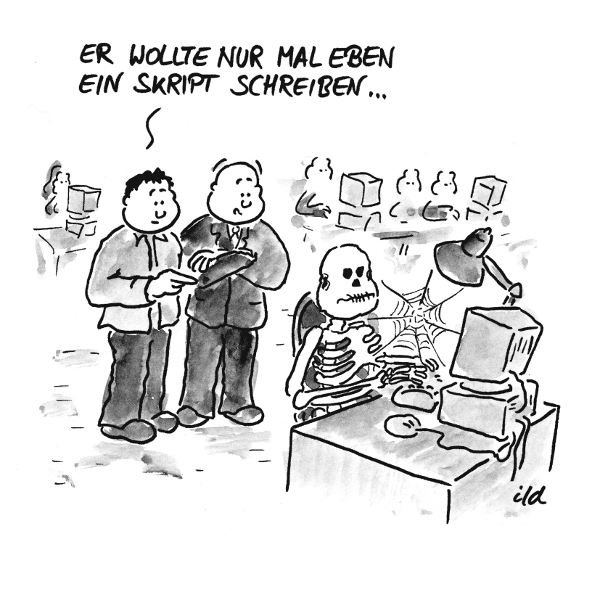
\includegraphics[width=0.5\textwidth]{Bilder/mal_eben_ein_skript_schreiben.jpg} %60% der Textbreite
\end{figure}
fangen wir mal recht einfach an.

\subsection{Den Spieler teleportieren}

Bei  dieser  Mission  untersuchst  du  die  Wirkungsweise  von  Variablen. 
Hierzu  teleportierst  du  deinen  Spieler  mithilfe  von  Integern  an  eine 
andere Position.
Ähm HALT STOPP was sind variablen und was ist ein Integer? 

Variablen gestatten dir das Speichern von Daten, die du an späterer Stelle im Programm  noch  einmal  brauchst. Daten können  dabei  alles  Mögliche  sein, was   gespeichert   werden   soll:   Zahlenwerte,   Namen,   beliebige  Texte, Objektlisten usw. Hier beispielsweise ist eine Variable namens juckel, die den Zahlenwert 3 speichert: 

\lstset{language=Python}
\lstset{frame=lines}
\lstset{caption={Insert code directly in your document}}
\lstset{label={lst:code_direct}}
\lstset{basicstyle=\footnotesize}
\begin{lstlisting}
juckel = 3
\end{lstlisting}

Integer sind positive oder negative ganze Zahlen. Werte wie 10, 32, -6, 194689 oder -5 sind Integer, Zahlen wie 3,14 und 6,025 jedoch nicht.

Um einen Spieler teleportieren zu wollen müssen wir zuerst verstehen wo er überhaupt steht und wo er hin soll. Im Spiel wird die Position oben links angezeigt:

\begin{figure}[H]
	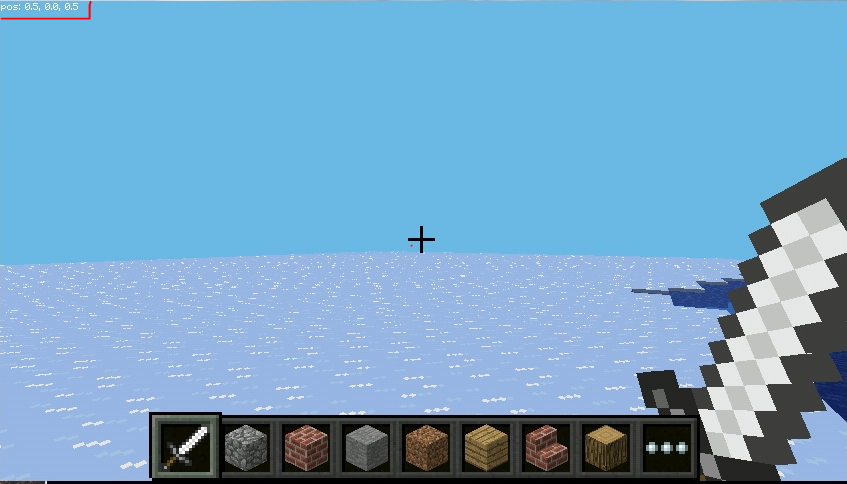
\includegraphics[width=0.5\textwidth]{Bilder/Mincraft_position.png} %60% der Textbreite
\end{figure}

Die drei Zahlen stehen für die x-, y- und z-Achse in einem dreidimensionalem Raum. Im folgendem Bild ist dieser dargestellt. Jeder Pfeil stellt eine Richtung dar in welche die Figur sich bewegen kann.
\begin{figure}[H]
	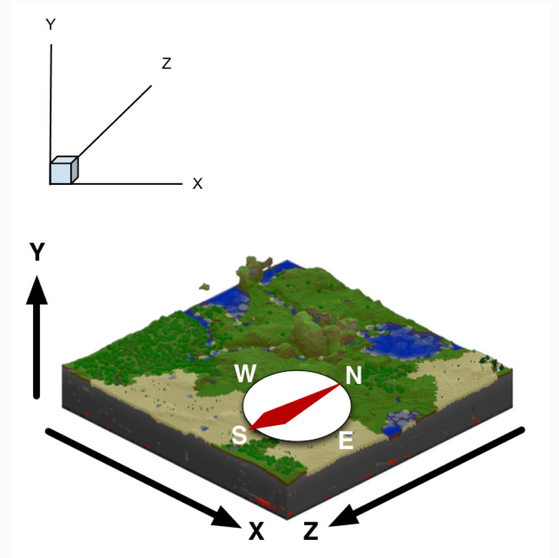
\includegraphics[width=0.5\textwidth]{Bilder/dreidimensionalem_Raum.png} %60% der Textbreite
\end{figure}

Bewege deinen Spieler im Spiel, und achte dabei darauf, wie sich die Positionszahlen verändern. Dies sollte beim Bewegen des Spielers in Echtzeit 
erfolgen. Eigentlich ganz cool, oder? Allerdings benötigt man hierbei für 
lange Wege viel Zeit. Deswegen lassen wir ihn teleportieren. Hierzu öffnen wir im Raspberry Pi das Programm Thonny Python IDE.
\begin{figure}[H]
	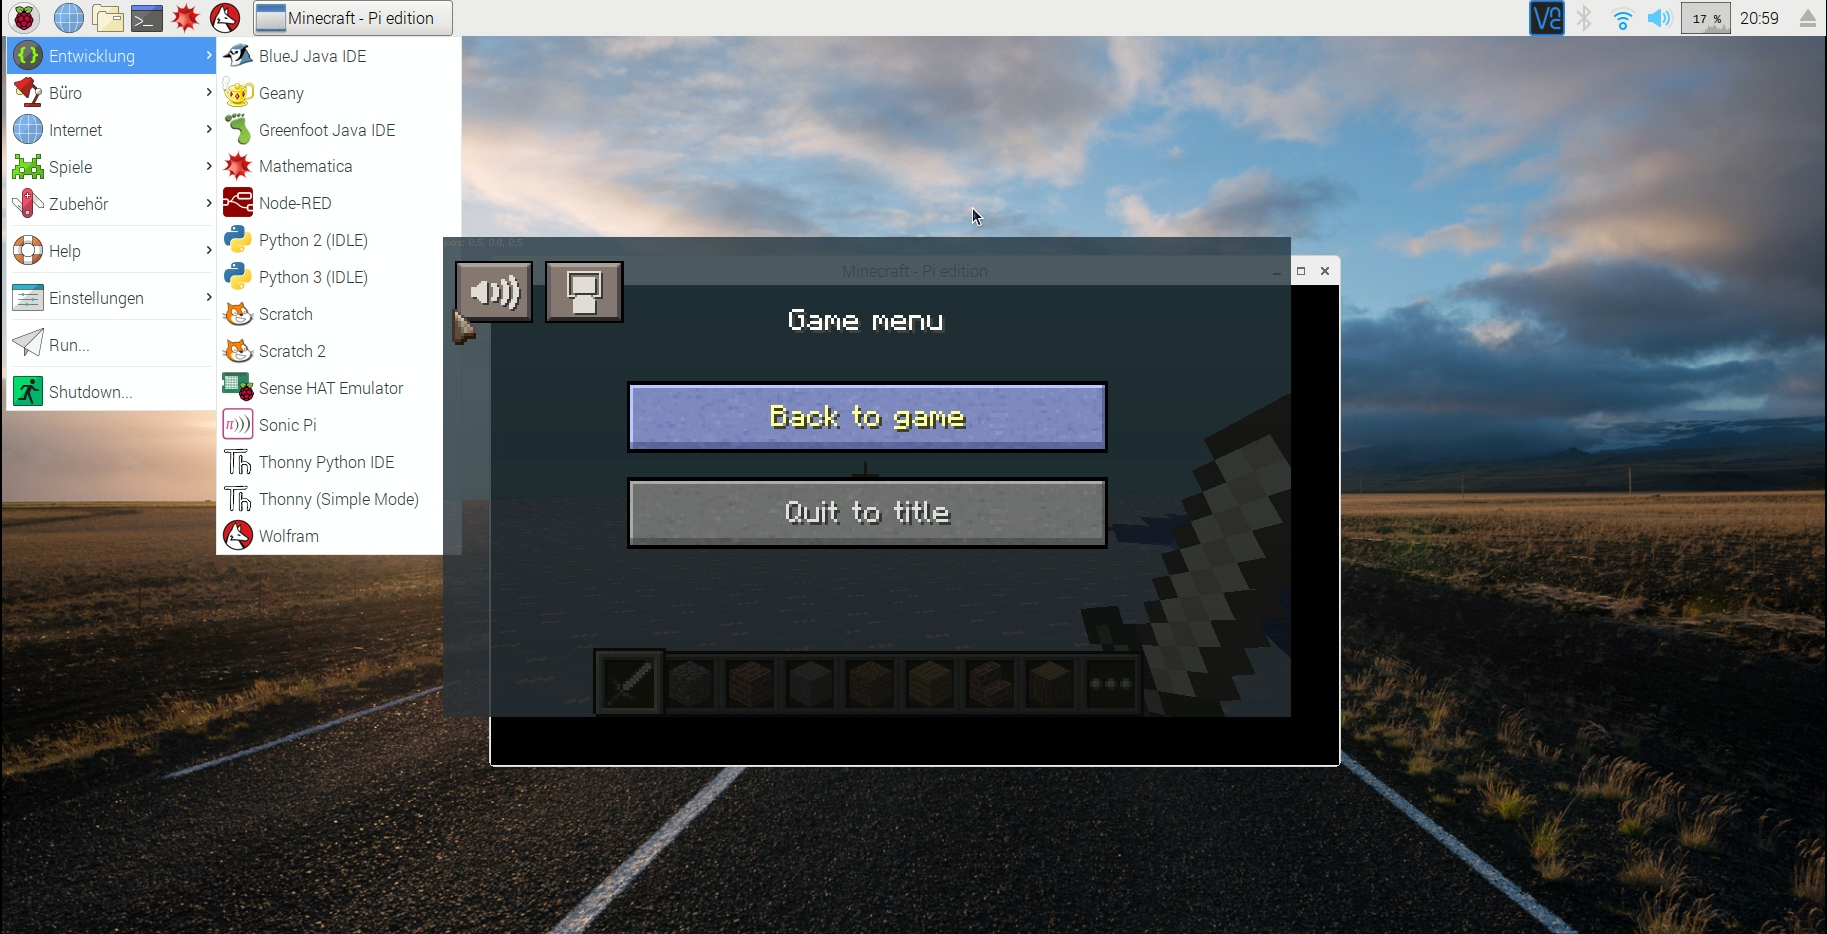
\includegraphics[width=0.5\textwidth]{Bilder/Thonny_Python_IDE.png} %60% der Textbreite
\end{figure}

Und ordnen den Programme wie folgt auf dem Bildschirm an:
\begin{figure}[H]
	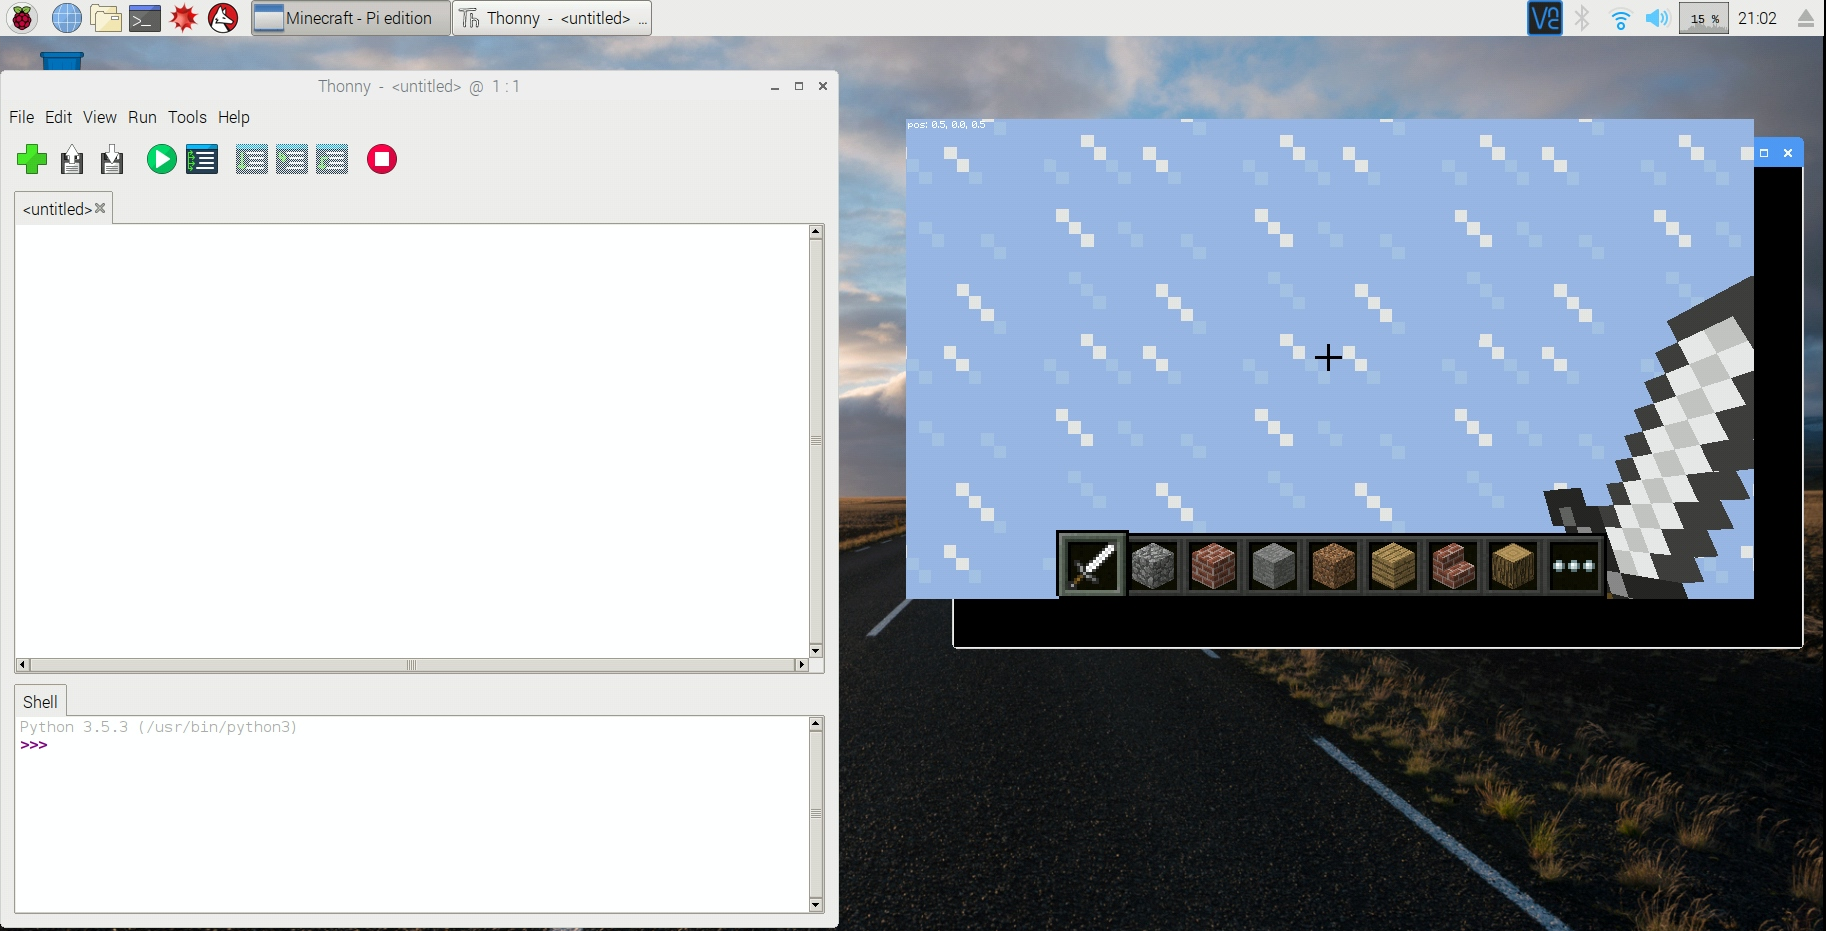
\includegraphics[width=0.5\textwidth]{Bilder/Bildschirm_Anordnung.png} %60% der Textbreite
\end{figure}

Nun schreiben wir in das linke Fenster unser erstes Programm. Dies sieht wie folgt aus:

\lstset{language=Python}
\lstset{frame=lines}
\lstset{caption={Insert code directly in your document}}
\lstset{label={lst:code_direct}}
\lstset{basicstyle=\footnotesize}
\begin{lstlisting}
# Verbindung mit Minecraft herstellen
from mcpi.minecraft import Minecraft
mc = Minecraft.create()

# Variablen x, y und z zur Darstellung
# der Koordinaten festlegen 
x = 10
y = 110
z = 12

# Position des Spielers aendern 
mc.player.setTilePos(x, y, z)
\end{lstlisting}


Wichtig ist hierbei damit die Zahlen Variablen x, y und z nicht größer als 127 und nicht kleiner als -127 sind. Nun sollte es wie folgt aussehen:

\begin{figure}[H]
	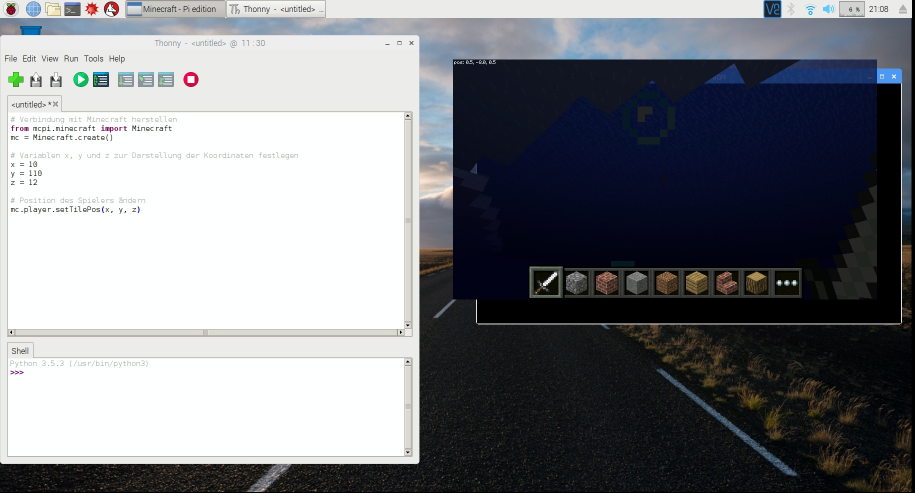
\includegraphics[width=0.5\textwidth]{Bilder/Erstes_Programm.png} %60% der Textbreite
\end{figure}
Drücken wir nun den grünen Kreis mit dem weißen Pfeil wird unser Programm ausgeführt und unserer Spieler wird auf die eingestellt Position gestellt. Es kann sein damit zuerst die Aufforderung kommt zum Speichern. Hier kannst du kreativ sein und ein Name vergeben.

Natürlich kannst du auch anstelle von Integer-Variablen auch Float-Variablen vergeben. Float-Variablen sind Zahlen mit Nachkommastellen, wie z.B. 1.34 (Wichtig für das Komma ein Punkt setzen, da man das so in England macht und beim Programmieren ist Englisch die Hauptsprache). Dann sieht unsere obiges Beispiel mit juckel so aus:
\lstset{language=Python}
\lstset{frame=lines}
\lstset{caption={Insert code directly in your document}}
\lstset{label={lst:code_direct}}
\lstset{basicstyle=\footnotesize}
\begin{lstlisting}
juckel = 1.34
\end{lstlisting}
Jetzt ist juckel eine Float-Variable. Mit Float-Variablen kann man sich punktgenau teleportieren, was natürlich auch mit negative Zahlen geht. 
\lstset{language=Python}
\lstset{frame=lines}
\lstset{caption={Insert code directly in your document}}
\lstset{label={lst:code_direct}}
\lstset{basicstyle=\footnotesize}
\begin{lstlisting}
juckel = -1.34
\end{lstlisting}

\subsection{Weiter wichtige Funktionen}


Mit dieser Funktion kannst du an Position x, y, z ein Block entfernen.
\lstset{language=Python}
\lstset{frame=lines}
\lstset{caption={Insert code directly in your document}}
\lstset{label={lst:code_direct}}
\lstset{basicstyle=\footnotesize}
\begin{lstlisting}
world.getBlock(x, y, z)
\end{lstlisting}

Mit dieser Funktion kannst du an Position x, y, z ein Block setzen.
\lstset{language=Python}
\lstset{frame=lines}
\lstset{caption={Insert code directly in your document}}
\lstset{label={lst:code_direct}}
\lstset{basicstyle=\footnotesize}
\begin{lstlisting}
world.setBlock(x, y, z, block_type)
\end{lstlisting}

 Wichtig ist damit du für block\_type einen der folgenden Block Namen einsetzt:
 AIR, STONE, GRASS, DIRT, COBBLESTONE, WOOD\_PLANKS, SAPLING, BEDROCK, WATER\_FLOWING, WATER, WATER\_STATIONARY, LAVA\_FLOWING, LAVA, LAVA\_STATIONARY, SAND, GRAVEL, GOLD\_ORE, IRON\_ORE, COAL\_ORE, WOOD, LEAVES, GLASS, LAPIS\_LAZULI\_ORE, LAPIS\_LAZULI\_BLOCK, SANDSTONE, BED, COBWEB, GRASS\_TALL, WOOL, FLOWER\_YELLOW, FLOWER\_CYAN, MUSHROOM\_BROWN, MUSHROOM\_RED, GOLD\_BLOCK, IRON\_BLOCK, STONE\_SLAB\_DOUBLE, STONE\_SLAB, BRICK\_BLOCK, TNT, BOOKSHELF, MOSS\_STONE, OBSIDIAN, TORCH, FIRE, STAIRS\_WOOD, CHEST, DIAMOND\_ORE, DIAMOND\_BLOCK, CRAFTING\_TABLE, FARMLAND, FURNACE\_INACTIVE, FURNACE\_ACTIVE, DOOR\_WOOD, LADDER, RAIL, STAIRS\_COBBLESTONE, DOOR\_IRON, REDSTONE\_ORE, SNOW, ICE, SNOW\_BLOCK, CACTUS, CLAY, SUGAR\_CANE, FENCE, GLOWSTONE\_BLOCK, BEDROCK\_INVISIBLE, STONE\_BRICK, GLASS\_PANE, MELON, FENCE\_GATE, GLOWING\_OBSIDIAN und NETHER\_REACTOR\_CORE.
 
 Mit dieser Funktion kannst du gleich mehrere Block auf einmal setzen. Hier Baut das Programm dir alles zu von x1 bis x2 und von y1 bis y2 und von z1 bis z2.

\lstset{language=Python}
\lstset{frame=lines}
\lstset{caption={Insert code directly in your document}}
\lstset{label={lst:code_direct}}
\lstset{basicstyle=\footnotesize}
\begin{lstlisting}
world.setBlocks(x1, y1, z1, x2, y2, z2, block_type)
\end{lstlisting}

Diese Funktion gibt dir den höchsten Block auf der Stelle x, z zurück. 

\lstset{language=Python}
\lstset{frame=lines}
\lstset{caption={Insert code directly in your document}}
\lstset{label={lst:code_direct}}
\lstset{basicstyle=\footnotesize}
\begin{lstlisting}
 world.getHeight(x, z)
\end{lstlisting}

Mit dieser Funktion kannst du Nachrichten schreiben im Spiel.

\lstset{language=Python}
\lstset{frame=lines}
\lstset{caption={Insert code directly in your document}}
\lstset{label={lst:code_direct}}
\lstset{basicstyle=\footnotesize}
\begin{lstlisting}
world.postToChat("Message")
\end{lstlisting}
